\begin{frame}{Library on GitHub}
\only<1>{
\note{
For our DDRF method, we have developed an R library. It is available on CRAN and on GitHub. You can access it using this QR code.

}

  \begin{center}

    \qrcode{https://github.com/Xaleed/DirichletRF.git}
 \end{center}
    
    \centering
    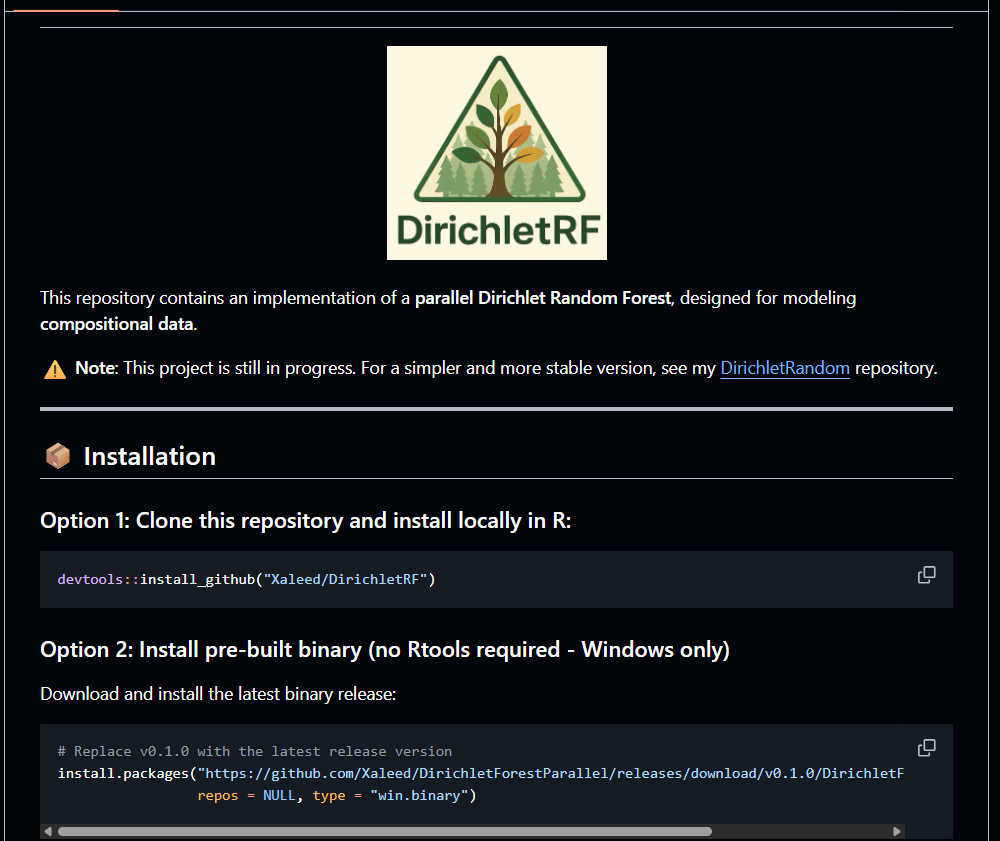
\includegraphics[width=0.45\linewidth]{slides/github.png}
    \caption{}
}
% \only<2>{
% \note{
% We developed an R library for this Random Forest model. This library implements the Random Forest in parallel and provides both predictions and empirical distributions. The parameters can be estimated using either Maximum Likelihood Estimation (MLE) or the Method of Moments (MoM), with MoM being the default option.

% }
%   \begin{center}

%     \qrcode{https://github.com/Xaleed/DirichletRF.git}
%  \end{center}
% %\vspace{0.3cm}

% \textbf{Key Features:}
% \begin{itemize}
% \item[\textcolor{blue}{\large$\blacktriangleright$}] Dirichlet distribution-based splits (likelihood maximization)
% \item[\textcolor{blue}{\large$\blacktriangleright$}] Parallel processing (Unix/Mac fork, Windows cluster)
% \item[\textcolor{blue}{\large$\blacktriangleright$}] Two purpose: Prediction vs. Distributional
% \item[\textcolor{blue}{\large$\blacktriangleright$}] Two parameter estimation methods (MoM, MLE)
% \end{itemize}


% }
    
\only<2>{
% \note{
% Most of the parameters are the same as in other well-known libraries. Here, we introduce two new parameters: \texttt{method} and \texttt{store\_samples}. I will briefly explain both.


% }
\begin{table}
\small
\begin{tabular}{lp{3cm}p{6cm}}
\toprule
\textbf{Parameter} & \textbf{Default} & \textbf{Description} \\
\midrule
\texttt{num.trees}  & 100          & Number of trees in the forest \\
\texttt{max.depth}  & 10           & Maximum tree depth \\
\texttt{min.node.size} & 5         & Minimum observations per leaf node \\
\texttt{mtry}       & $\sqrt{p}$   & Candidate features at each split \\
\texttt{seed}       & 123          & Random seed for the C++ RNG \\
\texttt{\textcolor{blue}{est.method}} & \texttt{"mom"} & Dirichlet estimation: \texttt{"mom"} or \texttt{"mle"} \\
\texttt{num.cores}  & $-1$         & OpenMP threads ($-1$ = all cores minus one) \\
\bottomrule
\end{tabular}
\end{table}
}
\end{frame}




% \begin{frame}{Conclusion}
%     \begin{itemize}

%     \item[\textcolor{blue}{\large$\blacktriangleright$}] 
%     \textbf{For compositional data}, we adapt Random Forest splitting rules to respect the geometry of the simplex, avoiding the limitations and potential bias introduced by traditional transformations to real space.
%     \vspace{1.1em}

%     \item[\textcolor{blue}{\large$\blacktriangleright$}] 
%     \textbf{Based on  comparison results, the model shows strong and stable performance}
%     across a wide range of scenarios.
%     \vspace{1.1em}

%     \item[\textcolor{blue}{\large$\blacktriangleright$}] 
%     \textbf{We also provide an open-source implementation} 
%     available as a Git/R package.
% \end{itemize}
% \end{frame}


